% !TeX root = project-report-en-concise.tex
% !TeX program = lualatex
% Build: latexmk -lualatex -interaction=nonstopmode -halt-on-error -outdir=.build/project-report-en-concise project-report-en-concise.tex
\documentclass[11pt,a4paper]{article}
\usepackage[margin=21mm,headheight=14pt]{geometry}
\usepackage{lmodern,amsmath,amssymb,graphicx,booktabs,array,tabularx}
\usepackage{xcolor,enumitem,fancyhdr,caption,xurl,placeins,float,needspace,titlesec}
\usepackage[colorlinks=true,linkcolor=teal,citecolor=teal,urlcolor=teal]{hyperref}
\definecolor{reportblue}{HTML}{18536B}
\hypersetup{pdftitle={Effects of Feature Groups on Four-Lepton MC Event Selection},pdfauthor={Hongyi Xu}}
\pagestyle{fancy}
\fancyhf{}
\fancyhead[L]{\small\textcolor{reportblue}{HiggsML | Progress report}}
\fancyhead[R]{\small Revised 15 November 2026}
\fancyfoot[C]{\thepage}
\setlength{\parindent}{0pt}
\setlength{\parskip}{5pt}
\setlength{\emergencystretch}{2em}
\setlist[itemize]{leftmargin=1.4em,itemsep=3pt,topsep=4pt}
\captionsetup{font=small,labelfont=bf,justification=raggedright,singlelinecheck=false}
\newcolumntype{Y}{>{\raggedright\arraybackslash}X}
\titleformat{\section}{\Large\bfseries\color{reportblue}}{\thesection}{1em}{}
\titleformat{\subsection}{\large\bfseries\color{reportblue}}{\thesubsection}{1em}{}
\titlespacing*{\section}{0pt}{16pt}{8pt}
\titlespacing*{\subsection}{0pt}{12pt}{5pt}
\raggedbottom
\widowpenalty=10000
\setlength{\textfloatsep}{12pt}
\setlength{\intextsep}{12pt}
\newcommand{\gev}{\,\mathrm{GeV}}

\begin{document}
{\LARGE\bfseries\color{reportblue} Effects of Feature Groups on\\ Four-Lepton MC Event Selection\par}
\vspace{6pt}
Hongyi Xu\par
Progress report $\cdot$ Revised 15 November 2026

\section{Purpose and scope}
This report compares five input configurations for neural-network selection of simulated $H\to ZZ^*\to4\ell$ events.
ABCD uses all groups; the other four configurations each remove one group.
Each configuration is trained with seeds 42, 43 and 44, giving fifteen models. All use the same event split, hidden layers and threshold rule.
The comparison uses signal retention, background retention and S/B; ABCD and BCD mass spectra show how selection changes the mass distribution.

Removing group C, which contains the four-lepton transverse momentum and the azimuthal separation between the two lepton pairs, lowers signal retention, raises background retention and lowers S/B in all three seeds.
The median decrease in signal retention is 3.94 percentage points. Other deletions give mixed results.
This is an educational, exploratory MC study.
Numerical values are retained from the previously checked result record. The retained tables can be checked for internal consistency, but the complete historical result package and its source bindings cannot currently be reverified locally.

\section{Samples and event weights}
The inputs are ATLAS 2020 educational 13 TeV MC samples~\cite{OpenData}.
Signal is DSID 345060 (\texttt{ggH125\_ZZ4lep}); background is DSID 363490 (\texttt{llll}).
The signal models gluon-fusion production of a $125\gev$ Higgs followed by $H\to ZZ^*\to4\ell$.
Background means only the selected \texttt{llll} sample, not the full experimental background.
The \href{https://opendata.cern.ch/record/15005}{CERN release page} lists the files; Appendix~\ref{app:mc-generation} explains MC generation and the missing production details.

Both samples pass the same trigger, lepton-quality, momentum, acceptance and pair-mass cuts (Appendix~\ref{app:cuts}).
The final state is $2e2\mu$ with $105\leq m_{4\ell}<140$ GeV. The electron or muon pair closer to $91.1876$ GeV is $Z_1$; the other is $Z_2$.
``Before network selection'' means all final-evaluation events passing these cuts. ``After selection'' means their high-score subset.

Physical event groups are assigned with the probabilities below. Related records stay together, and every model uses the same assignment.
\begin{center}
\small
\begin{tabularx}{\linewidth}{@{}p{.18\linewidth}p{.19\linewidth}Y@{}}
\toprule
Subset & Allocation probability & Role \\
\midrule
Training & 60\% & Fit input-standardization and network parameters. \\
Validation & 20\% & Select a checkpoint using AUC, then determine a threshold from background scores. \\
Final evaluation & 20\% & Calculate selected yields and mass spectra after freezing the model and threshold. \\
\bottomrule
\end{tabularx}
\end{center}

\begin{table}[H]
\caption{Input-file entries and final-evaluation counts. Physical cuts and allocation both separate the two rows.}
\label{tab:population}
\centering\small
\begin{tabularx}{\linewidth}{@{}Y p{.23\linewidth} rrr@{}}
\toprule
Sample stage & Counting unit & Signal & Background & Total \\
\midrule
Input MC samples & File entries & 164,716 & 554,279 & 718,995 \\
Final evaluation (before selection) & Distinct physical events & 9,049 & 698 & 9,747 \\
\bottomrule
\end{tabularx}
\end{table}

\subsection{Physical weights and yields}\label{sec:weights}
Counts describe simulation records or groups. Nominal MC yields sum signed physical weights at the target luminosity $10\,\mathrm{fb}^{-1}$:
\[
 w_i^{\rm phys}=\frac{\mathcal L\,\sigma_{\rm eff}}{S_{\rm gen}}\,w_i^{\rm gen},
 \qquad \mathcal L=10^4\,\mathrm{pb}^{-1}.
\]
Here $w_i^{\rm gen}$ is the stored generator weight, $\sigma_{\rm eff}$ is the effective cross section, and $S_{\rm gen}$ is the generator-weight sum.
The pinned official table~\cite{SampleInfo} agrees with the configuration:
\begin{center}
\small
\begin{tabular}{lrr}
\toprule
Sample & $\sigma_{\rm eff}$ ($\mathrm{pb}$) & $S_{\rm gen}$ \\
\midrule
Signal & 0.0060239 & 27881776.6536 \\
Background & 1.2578 & 7538705.8077 \\
\bottomrule
\end{tabular}
\end{center}
The evaluation weight corrects for its allocation probability:
\[
 u_i=\frac{w_i^{\rm phys}}{0.2}.
\]
For the evaluation events $E$ of one process, score $s_i$ and frozen threshold $t$,
\[
 Y_{\rm before}=\sum_{i\in E}u_i,\qquad
 Y_{\rm high}=\sum_{i\in E,\,s_i\geq t}u_i.
\]
Negative weights retain their signs. These nominal MC yields use simplified normalization without pileup, lepton or trigger scale factors (Appendix~\ref{app:normalization}).

\textbf{Illustration only (not study data).}
Consider three distinct evaluation events from a hypothetical process with $\sigma_{\rm eff}=0.01\,\mathrm{pb}$ and $S_{\rm gen}=1000$ for the full generated sample.
At the same $\mathcal L=10^4\,\mathrm{pb}^{-1}$, the normalization factor is $\mathcal L\sigma_{\rm eff}/S_{\rm gen}=0.1$.
This scales generator weights to the nominal event rate at the target luminosity. Dividing by 0.2 then compensates for using only the evaluation subset.
\begin{center}
\small
\begin{tabular}{lrrr}
\toprule
Event & Generator weight $w_i^{\rm gen}$ & Physical weight $w_i^{\rm phys}$ & Evaluation weight $u_i$ \\
\midrule
1 & $1$ & $0.1$ & $0.5$ \\
2 & $2$ & $0.2$ & $1.0$ \\
3 & $-0.5$ & $-0.05$ & $-0.25$ \\
\bottomrule
\end{tabular}
\end{center}
The three events give $Y_{\rm before}=0.5+1.0-0.25=1.25$.
If only events 1 and 3 pass the score threshold, $Y_{\rm high}=0.5-0.25=0.25$.
The selected count is two events, while their nominal MC yield is 0.25; each simulated event contributes its weight rather than one expected event.

\section{Network and threshold}
The inputs are grouped as follows. None explicitly includes $m_{4\ell}$, although the other variables can still carry mass information.
\begin{table}[H]
\caption{Input groups. ABCD, BCD, ACD, ABD and ABC have 19, 11, 15, 17 and 14 inputs, respectively.}
\label{tab:feature-overview}
\centering\small
\begin{tabularx}{\linewidth}{@{}cp{.36\linewidth}Yc@{}}
\toprule
Group & Variables & Physical meaning & Dim. \\
\midrule
A & Four leptons' $p_T$, $\eta$ & Single-lepton momentum scale and direction & 8 \\
B & $m_{Z1}$, $m_{Z2}$, within-pair $\Delta R$ & Pair masses and internal angular separation & 4 \\
C & $p_{T,4\ell}$, $|\Delta\phi_{ZZ}|$ & Overall transverse motion and azimuthal relation between pairs & 2 \\
D & Three angle cosines and two plane angles & Production and decay orientations & 5 \\
\bottomrule
\end{tabularx}
\end{table}

\subsection{Model and training}\label{sec:network}
Each input $x_{ij}$ is standardized using only its training mean $\mu_j$ and standard deviation $\sigma_j$:
\[
 \widetilde x_{ij}=\frac{x_{ij}-\mu_j}{\sigma_j}.
\]
The same statistics are used for validation and evaluation; a zero standard deviation is replaced by 1.
The PyTorch MLP has this structure:
\[
 \underbrace{d_{\rm in}}_{\text{input}}
 \;\longrightarrow\;
 \underbrace{64\;\longrightarrow\;64\;\longrightarrow\;32}_{\text{three hidden layers}}
 \;\longrightarrow\;
 \underbrace{1}_{\text{output}}.
\]
\begin{table}[H]
\caption{Network operations. Only the input dimension changes between configurations.}
\label{tab:network}
\centering\small
\begin{tabularx}{\linewidth}{@{}p{.20\linewidth}p{.18\linewidth}Y@{}}
\toprule
Component & Dimensions & Operations in order \\
\midrule
Input processing & $d_{\rm in}\to d_{\rm in}$ & Standardize each input using its training-set mean and standard deviation. \\
Hidden layer 1 & $d_{\rm in}\to64$ & Linear, LayerNorm, SiLU, Dropout (0.1). \\
Hidden layer 2 & $64\to64$ & Linear, LayerNorm, SiLU, Dropout (0.1). \\
Hidden layer 3 & $64\to32$ & Linear, LayerNorm, SiLU. \\
Output & $32\to1$ & Linear produces a real value $z$; sigmoid is applied when computing the score. \\
\bottomrule
\end{tabularx}
\end{table}
A fully connected node combines previous outputs $h_k$ with learned weights $W_{jk}$ and bias $b_j$:
\[
 a_j=\sum_k W_{jk}h_k+b_j.
\]
The real output $z$ gives score
\[
 s=\frac{1}{1+e^{-z}}
\]
Higher scores are more signal-like. Class rescaling during training means the score is not a calibrated signal probability.

Signal has label $y_i=1$ and background $y_i=0$. The per-event loss is
\[
 \ell_i=-\left[y_i\ln s_i+(1-y_i)\ln(1-s_i)\right].
\]
For signal, the loss is $-\ln s_i$, so a higher predicted score reduces it.
For background, the loss is $-\ln(1-s_i)$, so a lower score reduces it.
Training uses nonnegative optimization weights, with mean 1 within each class:
\[
 \overline w_c=\frac{1}{N_c}\sum_{i\in\mathcal T_c}|w_i^{\rm phys}|,
 \qquad
 \alpha_i=\frac{|w_i^{\rm phys}|}{\overline w_{y_i}}.
\]
$\mathcal T_c$ contains the $N_c$ training events of class $c=0,1$; class totals need not be equal.
For a batch $\mathcal B$ of $m$ events,
\[
 L_{\rm batch}=\frac{1}{m}\sum_{i\in\mathcal B}\alpha_i\ell_i.
\]
Events are shuffled each epoch into batches of at most 1024.
Backpropagation computes the gradient of the batch loss with respect to each parameter, describing how a small parameter change affects the loss.
AdamW combines running averages of gradients and their squares to adapt updates for each parameter.
Its learning rate $10^{-3}$ sets the overall step size. Weight decay $10^{-4}$ applies separate shrinkage toward zero to discourage large parameter values.
The seed controls initialization, shuffling and Dropout.

AUC is the area under the receiver operating characteristic curve and summarizes ranking across score thresholds.
It measures how often a signal event ranks above a background event, with half credit for ties; here it uses absolute physical weights.
AUC 0.5 corresponds to chance ranking and 1 to perfect separation.
The checkpoint is saved only when validation absolute-weight AUC improves by more than $10^{-4}$.
Training stops after 20 epochs without improvement or at 200 epochs, then restores the best checkpoint.
ABCD seed 42 stopped at epoch 87 and uses epoch 67; BCD stopped at 86 and uses 66.

\subsection{Threshold and evaluation}\label{sec:threshold}
Each model sets its threshold to the weighted median of its validation-background scores, using absolute physical weights.
It takes the first ordered score whose cumulative weight reaches half the total, without interpolation.
Scores $s\geq t$ enter the high category, including all ties; scores $s<t$ enter the low category.
ABCD and BCD seed-42 thresholds are $0.746724$ and $0.860891$. Their sizes are not performance measures because score scales differ.

Standardization, checkpoints and thresholds are frozen before evaluation. Evaluation events never select them.
Dropout is off during validation and evaluation. Each deletion retrains the network and resets the threshold.
Changing input dimension also changes the first-layer parameter count.
The comparison therefore measures the effect of refitting the selection procedure; correlated inputs prevent interpretation as independent physical contributions.

\section{Metrics and worked example}\label{sec:basic}
ABCD uses all groups; BCD removes A. Their seed-42 event counts are:
\begin{table}[H]
\caption{Physical event groups in final evaluation and the two high-score subsets.}
\label{tab:groups}
\centering
\begin{tabular}{lrrr}
\toprule
Process & Before selection & ABCD high score & BCD high score \\
\midrule
Signal & 9,049 & 8,761 & 8,563 \\
Background & 698 & 386 & 378 \\
\bottomrule
\end{tabular}
\end{table}

For signal and background evaluation sets $E_S,E_B$ and weights $u_i$, the common yields are
\[
 S_0=\sum_{i\in E_S}u_i,\qquad
 B_0=\sum_{i\in E_B}u_i.
\]
Selected yields are
\[
 S=\sum_{i\in E_S,\,s_i\geq t}u_i,\qquad
 B=\sum_{i\in E_B,\,s_i\geq t}u_i.
\]
The metrics are
\[
 R_S=\frac{S}{S_0},\qquad R_B=\frac{B}{B_0},\qquad Q=\frac{S}{B}.
\]
$R_S$ and $R_B$ are signed-yield retention fractions; background rejection is $1-R_B$.
For a common baseline,
\[
 Q=\frac{S_0}{B_0}\frac{R_S}{R_B}.
\]
Thus S/B is determined by the two retention fractions. A higher S/B can accompany signal loss and does not alone establish better sensitivity or precision.
Thresholds are not adjusted to equalize retention across models.
If $S_0$ or $B_0$ is nonpositive, its retention is undefined; S/B is undefined for $B\leq0$.
Negative yields and retention outside $[0,1]$ are retained and flagged.

\begin{table}[H]
\caption{Nominal signed MC yields at $10\,\mathrm{fb}^{-1}$ using the simplified normalization in Section~\ref{sec:weights}. Errors are grouped MC standard errors at fixed networks and thresholds; retention errors include shared-event covariance (Appendix~\ref{app:errors}).}
\label{tab:yields}
\centering
\begin{tabular}{llrr}
\toprule
Process & Selection & Nominal MC yield & Retention (\%) \\
\midrule
Signal & Before selection ($S_0$) & $2.7710\pm0.0293$ & --- \\
 & ABCD high score & $2.6824\pm0.0288$ & $96.80\pm0.19$ \\
 & BCD high score & $2.6215\pm0.0285$ & $94.60\pm0.24$ \\
Background & Before selection ($B_0$) & $2.3553\pm0.1683$ & --- \\
 & ABCD high score & $1.2027\pm0.1202$ & $51.06\pm3.57$ \\
 & BCD high score & $1.1012\pm0.1156$ & $46.75\pm3.57$ \\
\bottomrule
\end{tabular}
\end{table}

\begin{table}[H]
\caption{Seed-42 calculations and BCD minus ABCD differences. Calculations use displayed values; full results used unrounded yields. Retention differences are percentage points (pp).}
\label{tab:worked-metrics}
\centering\small
\renewcommand{\arraystretch}{2.6}
\begin{tabular}{lccr}
\toprule
Metric & ABCD & BCD & BCD $-$ ABCD \\
\midrule
Signal retention $R_S$ & $\dfrac{2.6824}{2.7710}\simeq96.80\%$ & $\dfrac{2.6215}{2.7710}\simeq94.60\%$ & $-2.20$ pp \\
Background retention $R_B$ & $\dfrac{1.2027}{2.3553}\simeq51.06\%$ & $\dfrac{1.1012}{2.3553}\simeq46.75\%$ & $-4.31$ pp \\
S/B $Q$ & $\dfrac{2.6824}{1.2027}\simeq2.23$ & $\dfrac{2.6215}{1.1012}\simeq2.38$ & $\simeq+0.15$ \\
\bottomrule
\end{tabular}
\end{table}
BCD loses signal but reduces background proportionally more, raising S/B. This example illustrates the tradeoff between signal retention and background suppression.

For removed group $G$ and seed $r$, contrasts always mean reduced minus ABCD:
\[
 \Delta R_{S,G,r}=R_S(\mathrm{ABCD}\setminus G,r)-R_S(\mathrm{ABCD},r),
\]
\[
 \Delta R_{B,G,r}=R_B(\mathrm{ABCD}\setminus G,r)-R_B(\mathrm{ABCD},r),\qquad
 \Delta Q_{G,r}=Q(\mathrm{ABCD}\setminus G,r)-Q(\mathrm{ABCD},r).
\]
Negative $\Delta R_S$ means less signal, negative $\Delta R_B$ less background, and positive $\Delta Q$ higher S/B.
All three seed differences enter each median and minimum--maximum range. Differences are calculated before taking medians.
The range describes seed variation and is not a confidence interval.

\section{Results}\label{sec:results}
All models share the same before-selection yields, $S_0=2.7710$ and $B_0=2.3553$.
For each model, the high- and low-score yields sum to these totals.
All fifteen models are reported below.

\begin{table}[H]
\caption{Results for all fifteen models. $R_S,R_B$ are percentages; $S,B$ are nominal MC yields at $10\,\mathrm{fb}^{-1}$.}
\label{tab:basic-all}
\centering\small
\begin{tabular}{llrrrrr}
\toprule
Inputs & Seed & $S$ & $B$ & $R_S$ & $R_B$ & $Q=S/B$ \\
\midrule
ABCD & 42 & 2.6824 & 1.2027 & 96.80 & 51.06 & 2.230 \\
ABCD & 43 & 2.6809 & 1.1589 & 96.75 & 49.20 & 2.313 \\
ABCD & 44 & 2.6670 & 1.0834 & 96.25 & 46.00 & 2.462 \\
\addlinespace
BCD & 42 & 2.6215 & 1.1012 & 94.60 & 46.75 & 2.381 \\
BCD & 43 & 2.6156 & 1.1145 & 94.39 & 47.32 & 2.347 \\
BCD & 44 & 2.6264 & 1.1344 & 94.78 & 48.16 & 2.315 \\
\addlinespace
ACD & 42 & 2.6667 & 1.1536 & 96.24 & 48.98 & 2.312 \\
ACD & 43 & 2.6679 & 1.1232 & 96.28 & 47.69 & 2.375 \\
ACD & 44 & 2.7039 & 1.2813 & 97.58 & 54.40 & 2.110 \\
\addlinespace
ABD & 42 & 2.5731 & 1.2186 & 92.86 & 51.74 & 2.112 \\
ABD & 43 & 2.5408 & 1.2192 & 91.69 & 51.76 & 2.084 \\
ABD & 44 & 2.5805 & 1.2026 & 93.13 & 51.06 & 2.146 \\
\addlinespace
ABC & 42 & 2.6975 & 1.1241 & 97.35 & 47.73 & 2.400 \\
ABC & 43 & 2.6972 & 1.0311 & 97.33 & 43.78 & 2.616 \\
ABC & 44 & 2.6941 & 1.1386 & 97.22 & 48.34 & 2.366 \\
\bottomrule
\end{tabular}
\end{table}

\begin{table}[H]
\caption{Within-seed differences from ABCD, with medians and ranges over all three seeds. Retention differences are in pp; S/B differences are dimensionless.}
\label{tab:basic-deltas}
\centering\small
\begin{tabular}{llccccc}
\toprule
Removed & Metric & Seed 42 & Seed 43 & Seed 44 & Median & Min--max \\
\midrule
A & $\Delta R_S$ & $-2.20$ & $-2.35$ & $-1.47$ & $-2.20$ & $[-2.35,-1.47]$ \\
A & $\Delta R_B$ & $-4.31$ & $-1.88$ & $+2.17$ & $-1.88$ & $[-4.31,+2.17]$ \\
A & $\Delta Q$ & $+0.150$ & $+0.033$ & $-0.147$ & $+0.033$ & $[-0.147,+0.150]$ \\
\addlinespace
B & $\Delta R_S$ & $-0.57$ & $-0.47$ & $+1.33$ & $-0.47$ & $[-0.57,+1.33]$ \\
B & $\Delta R_B$ & $-2.09$ & $-1.51$ & $+8.40$ & $-1.51$ & $[-2.09,+8.40]$ \\
B & $\Delta Q$ & $+0.081$ & $+0.062$ & $-0.351$ & $+0.062$ & $[-0.351,+0.081]$ \\
\addlinespace
C & $\Delta R_S$ & $-3.94$ & $-5.05$ & $-3.12$ & $-3.94$ & $[-5.05,-3.12]$ \\
C & $\Delta R_B$ & $+0.68$ & $+2.56$ & $+5.06$ & $+2.56$ & $[+0.68,+5.06]$ \\
C & $\Delta Q$ & $-0.119$ & $-0.229$ & $-0.316$ & $-0.229$ & $[-0.316,-0.119]$ \\
\addlinespace
D & $\Delta R_S$ & $+0.54$ & $+0.59$ & $+0.98$ & $+0.59$ & $[+0.54,+0.98]$ \\
D & $\Delta R_B$ & $-3.34$ & $-5.42$ & $+2.34$ & $-3.34$ & $[-5.42,+2.34]$ \\
D & $\Delta Q$ & $+0.169$ & $+0.302$ & $-0.096$ & $+0.169$ & $[-0.096,+0.302]$ \\
\bottomrule
\end{tabular}
\end{table}

\begin{figure}[H]
\centering
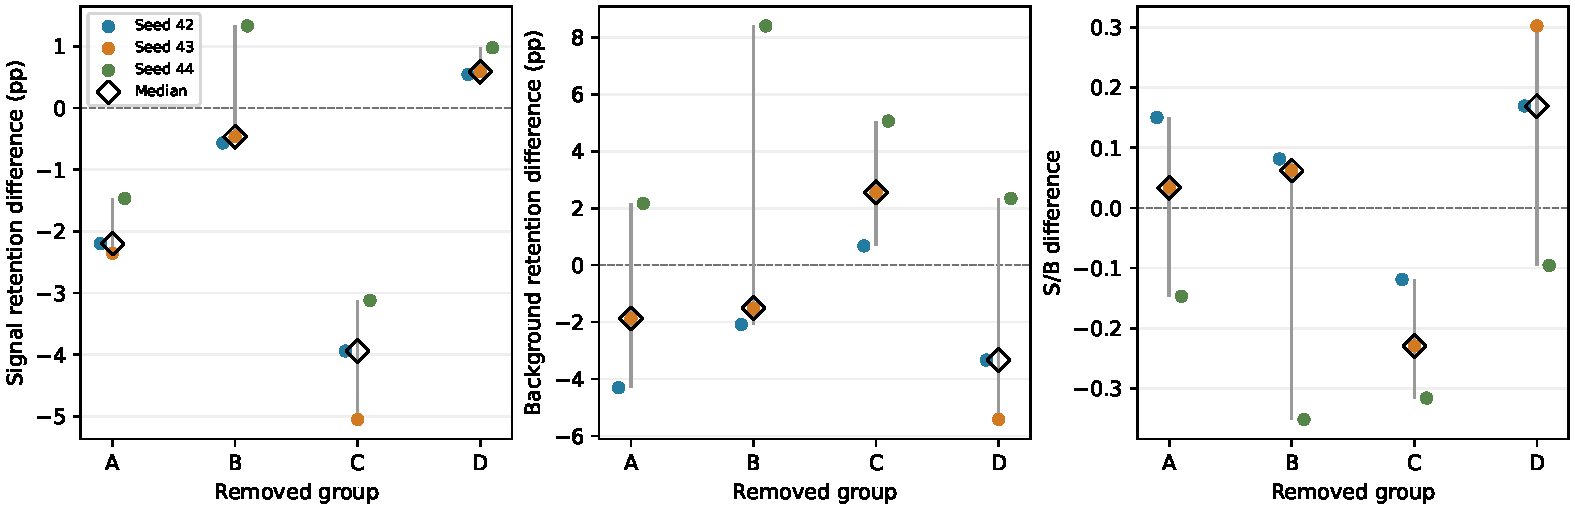
\includegraphics[width=\linewidth]{figures/basic-20261108/deletion-differences.pdf}
\caption{Deletion differences relative to ABCD. Circles show seeds 42--44, diamonds the medians and lines the minimum--maximum ranges. Dashed lines mark zero. Ranges are not confidence intervals.}
\label{fig:basic-deltas}
\end{figure}

\textbf{Removing C} gives signal-retention differences of $-5.05$ to $-3.12$ pp, background-retention differences of $+0.68$ to $+5.06$ pp and S/B differences of $-0.316$ to $-0.119$.
ABCD therefore retains more signal and less background than ABD in each seed. C's two variables were not removed separately, so their individual roles are unknown.

\textbf{Removing A} lowers signal retention in every seed ($-2.35$ to $-1.47$ pp). Seeds 42 and 43 reduce background and raise S/B; seed 44 does the reverse.
\textbf{Removing B} gives sign changes across seeds in all three deletion differences: seeds 42 and 43 retain slightly less signal and background with higher S/B, while seed 44 retains more of both with lower S/B.
\textbf{Removing D} raises signal retention in every seed ($+0.54$ to $+0.98$ pp), but background and S/B improve only in seeds 42 and 43; seed 44 reverses those directions.

Only removal of C consistently loses signal and retains more background. The other deletions do not give a consistent ordering.
Statistical significance of these differences was not assessed. Their uncertainties, including correlations from shared evaluation events, were not estimated.

\Needspace{8\baselineskip}
\section{Mass spectra}
The spectra illustrate how selection changes the mass distribution for ABCD and BCD seed 42, using seven 5 GeV bins.
Retention and S/B still use the full $[105,140)$ GeV window.
For each process and bin $b$,
\[
 Y_b=\sum_{i\in b}u_i.
\]
Before-selection sums use all evaluation events; selected sums use high-score events. Bin sums equal the corresponding total yield.

\begin{figure}[H]
\centering
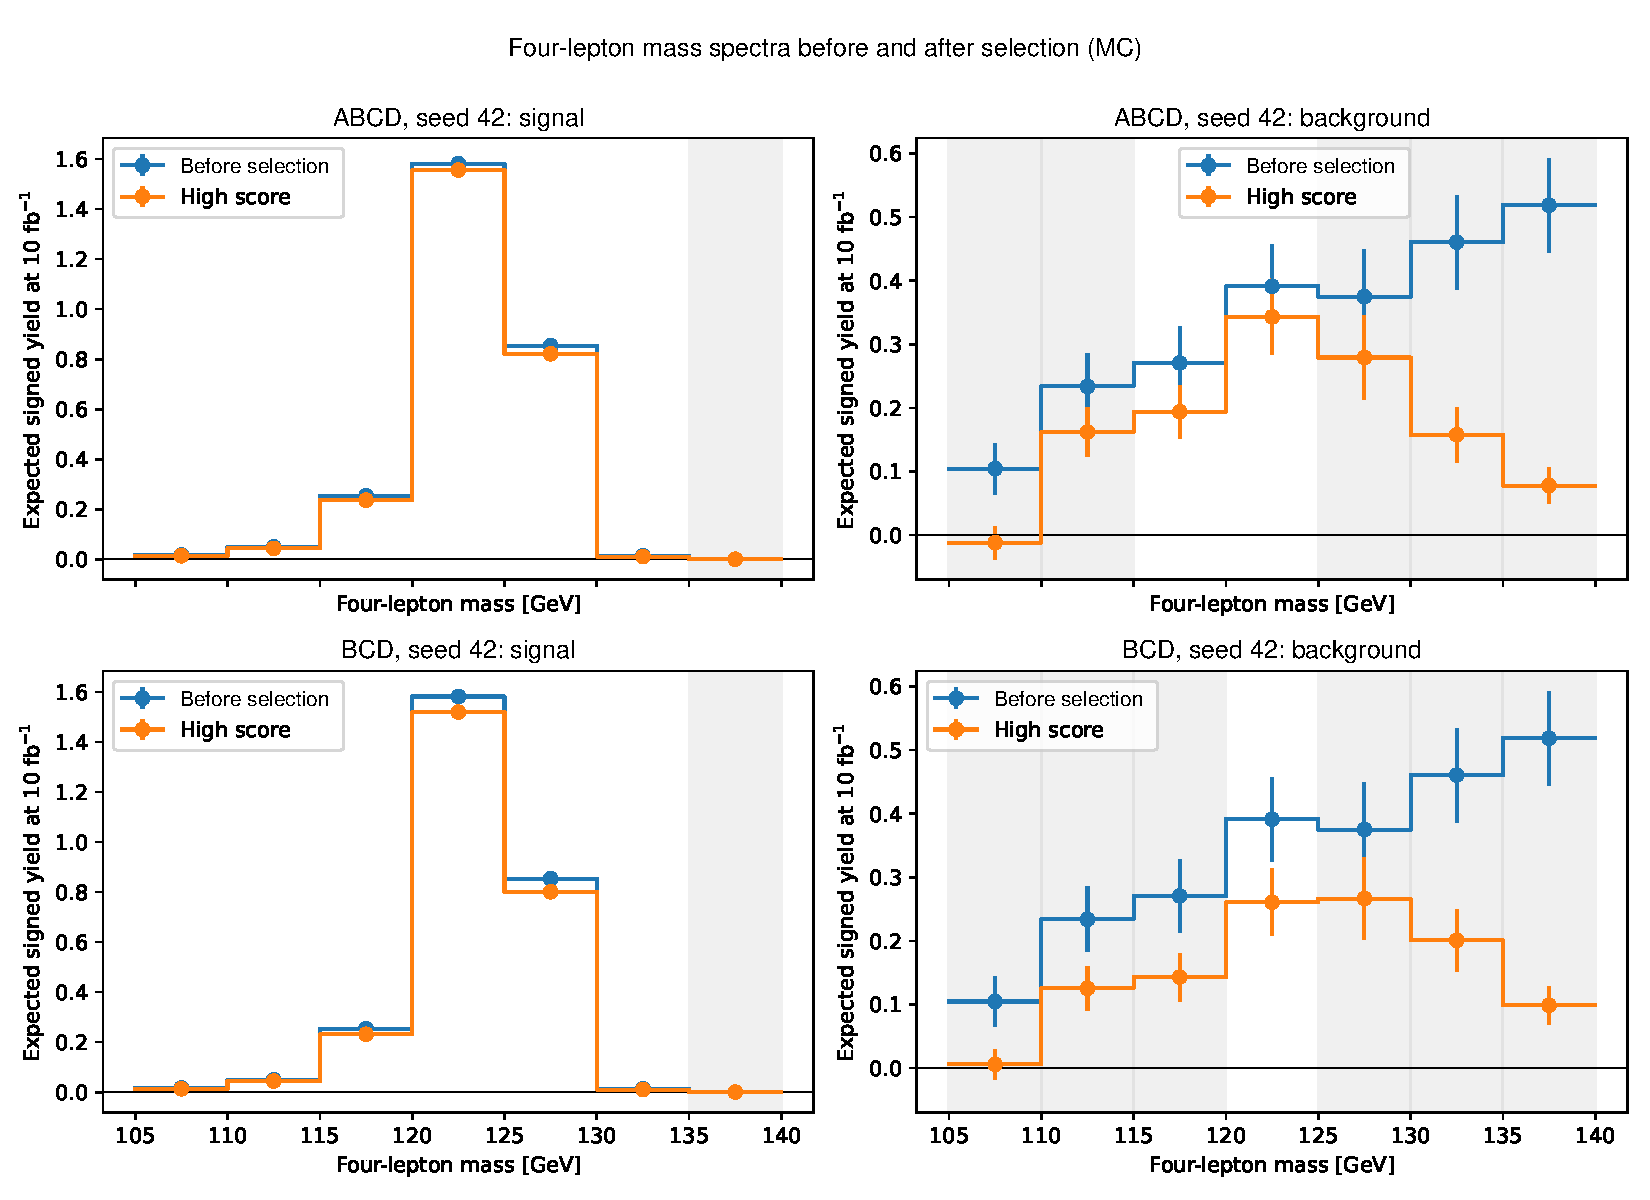
\includegraphics[width=.98\linewidth]{figures/report-en-20261115/mass-yields.pdf}
\caption{Nominal signed MC yields at $10\,\mathrm{fb}^{-1}$: ABCD above BCD, signal left and background right. Blue shows before-selection yields; orange shows high-score yields. Steps show 5 GeV bins, with points and grouped MC standard errors at bin centres. Shading flags limited support; negative yields are retained. Signal/background scales differ.}
\label{fig:yields}
\end{figure}
Signal remains concentrated near 125 GeV. Selection changes which events remain while keeping their masses fixed.
The coarse bins are not used to infer changes in peak position, detector resolution or intrinsic width.
Background covers the window nonuniformly, with a stronger reduction in the high-mass tail.

For a positive total $Y_{\rm total}=\sum_bY_b$, the normalized share is
\[
 f_b=\frac{Y_b}{Y_{\rm total}}.
\]
Each curve uses its own total, subject to the support conditions in Appendix~\ref{app:shape-support}.
Signed shares can be negative, so these curves need not be probability densities.

\begin{figure}[H]
\centering
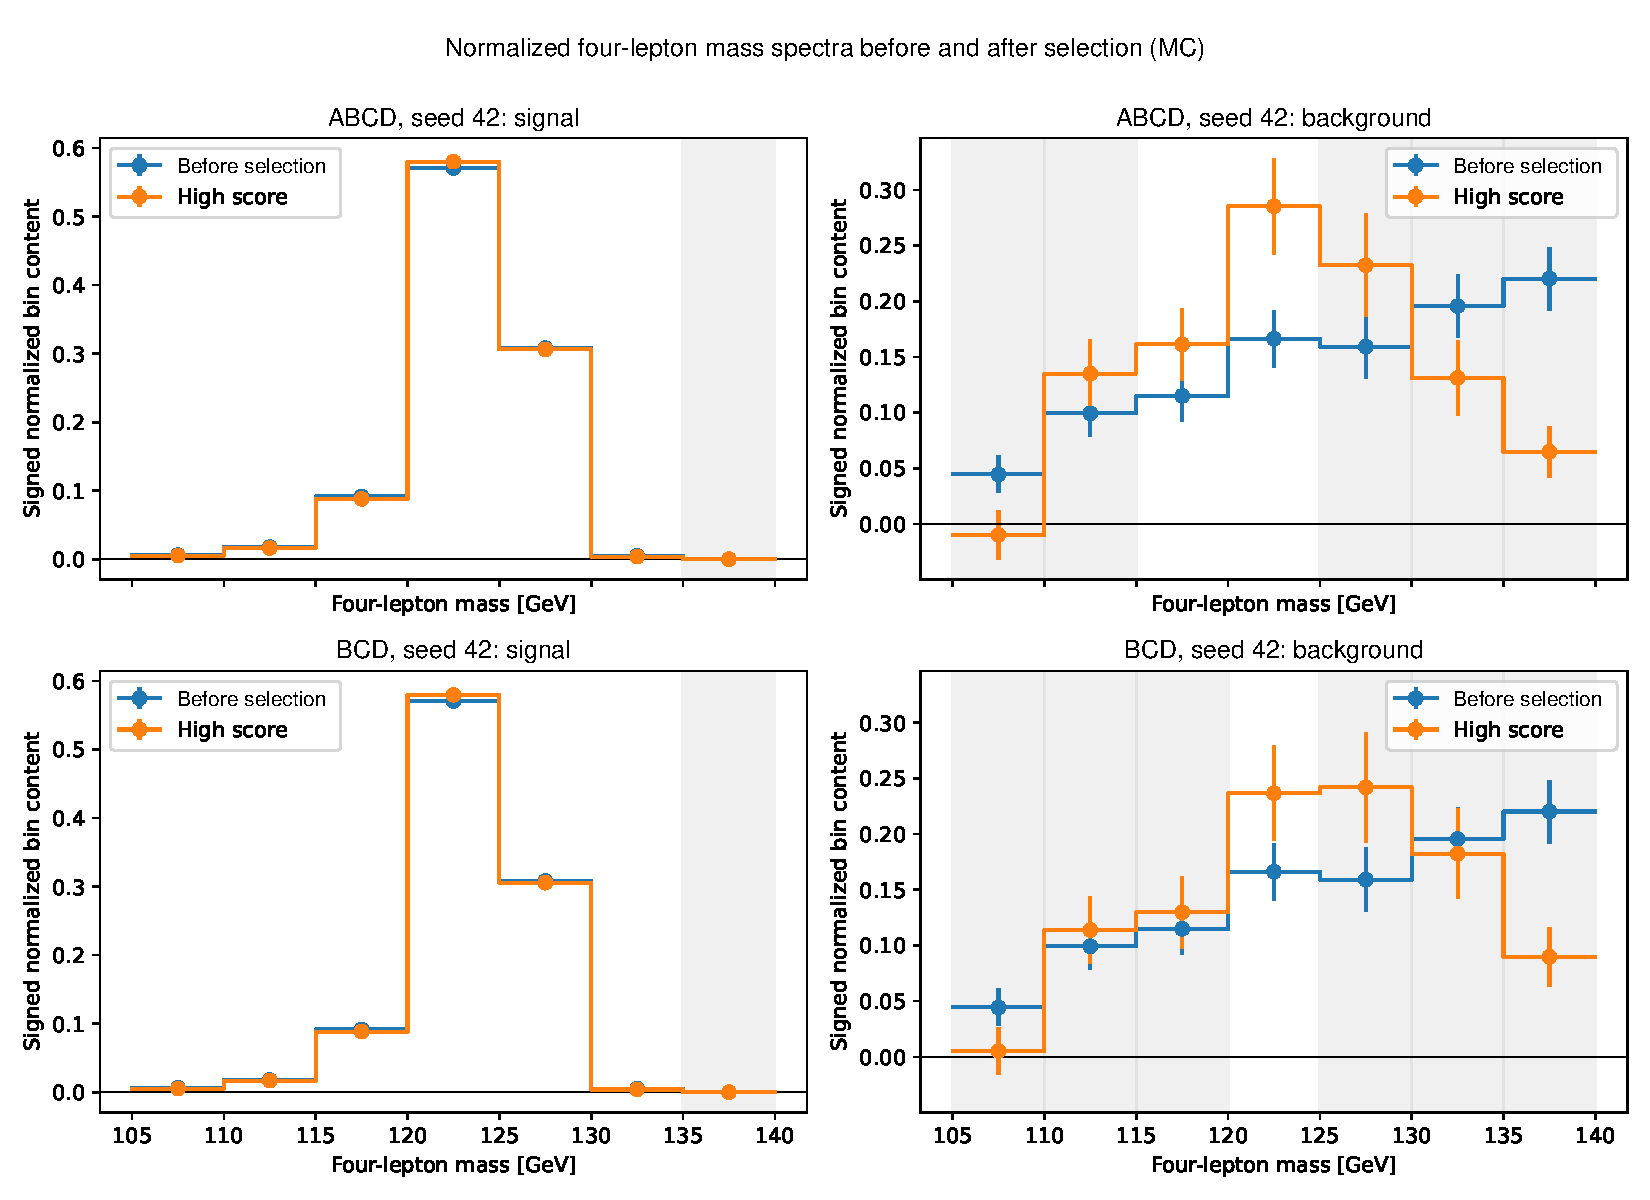
\includegraphics[width=.96\linewidth]{figures/report-en-20261115/mass-shapes.pdf}
\caption{Separately normalized spectra for the same events and thresholds as Figure~\ref{fig:yields}. Errors include shared normalization. Before/after curves share events, and bins are correlated. No smoothing, clipping or rebinning is applied; shading and negative values remain.}
\label{fig:shapes}
\end{figure}

\begin{table}[H]
\caption{Regional shares of each curve's signed total (\%). Differences are descriptive; their uncertainties are not shown.}
\label{tab:fractions}
\centering\small
\begin{tabular}{llrrr}
\toprule
Process & Region (GeV) & Before selection & ABCD high score & BCD high score \\
\midrule
Signal & $[120,130)$ & 87.9 & 88.6 & 88.5 \\
Background & $[120,130)$ & 32.5 & 51.8 & 47.9 \\
Background & $[135,140)$ & 22.0 & 6.5 & 9.0 \\
\bottomrule
\end{tabular}
\end{table}
The signal share changes little. Background becomes relatively more concentrated in $[120,130)$ GeV and less in $[135,140)$ GeV, even as its total falls.
A larger share does not imply a larger absolute regional yield.
The changes are consistent with mass-dependent selection despite omitting explicit $m_{4\ell}$.
This two-model example does not identify the responsible inputs or establish a background resonance.
ABCD high-score background is negative in $[105,110)$ GeV. Several background bins and the signal tail also have limited support (Appendix~\ref{app:errors}).

\Needspace{24\baselineskip}
\begin{samepage}
\section{Conclusions and next steps}\label{sec:conclusion}
Removing C lowers signal retention, raises background retention and lowers S/B in every recorded seed. Other deletions have seed-dependent tradeoffs.
The spectra show why total yields and mass shapes should be considered together.
These findings apply to the selected samples, network and threshold rule; the mass spectra cover only ABCD and BCD at one seed.

Seed ranges describe these training results; MC errors condition on fixed networks and thresholds.
Neither covers the full training and threshold uncertainty. The study does not evaluate measurement precision.
Production details, some cut references and physical normalization remain unresolved (Appendices~\ref{app:fields}, \ref{app:cuts} and~\ref{app:normalization}).
The analysis remains exploratory and non-independent; reusing or repartitioning the source events does not create independent validation. These are MC selection comparisons, not a physics measurement.

The first priority is to recover the exact historical result package and verify its source bindings.
The next task is to estimate paired uncertainties on the deletion differences, accounting for shared evaluation events and distinguishing them from training and threshold variation.
These tasks remain to be completed.
\end{samepage}

\setlength{\parskip}{4pt}
\appendix
\section{MC samples, fields and reconstruction}\label{app:fields}

\subsection{MC generation and its evidence limits}\label{app:mc-generation}
MC generators sample event kinematics from theoretical differential cross sections.
For idealized independent sampling from a nonnegative density,
\[
 p(x)=\frac{1}{\sigma}\frac{d\sigma}{dx},\qquad
 \int g(x)p(x)\,dx\simeq\frac{1}{N}\sum_{k=1}^{N}g(x_k),\quad x_k\sim p.
\]
$x$ denotes kinematics, $\sigma$ the integrated cross section, $g$ the event function and $N$ the sample size.
Actual generators can use importance sampling and weighted events; higher-order calculations and shower matching can produce signed weights. Negative weights alone do not identify their origin.

A typical chain generates hard scattering using parton distribution functions and perturbative calculations, then simulates showers, hadronization, decays and detector/trigger response before reconstructing objects~\cite{ATLASSimulation}.
This general description does not establish the settings of these two samples.
The project begins with ATLAS's released reconstructed leptons; it does not generate collisions or resimulate the detector.

The CERN record~\cite{OpenData} confirms the 2020 13 TeV collection and loose preselection with at least four electrons or muons.
The pinned parameter table~\cite{SampleInfo} gives DSIDs and normalization constants. Both input files match the recorded checksums, data structure and entry counts.
The remaining gaps are:
\begin{center}
\small
\begin{tabularx}{\linewidth}{@{}>{\raggedright\arraybackslash}p{.23\linewidth}Y@{}}
\toprule
Information & Scope and limitations of the source checks \\
\midrule
Sample identity & Signal DSID 345060 (\texttt{ggH125\_ZZ4lep}) and background DSID 363490 (\texttt{llll}) correspond to the 2020 dataset contract and public file list. \\
Generator and theory settings & DSID-specific production records are still needed for the generator/version, perturbative order, parton distribution functions, shower/hadronization settings, tune and generation filters. \\
Detector and object definitions & The inspected release record, parameter table and ROOT metadata do not establish the detector-simulation configuration, pileup, radiation treatment or exact lepton-object definitions. \\
Release preselection & Loose preselection is confirmed; exact momentum, acceptance and quality thresholds remain unverified. \\
Normalization and background composition & Parameter values can be checked; effective-cross-section factorization, negative-weight origin and the initial-state/interference composition of \texttt{llll} remain unresolved. \\
\bottomrule
\end{tabularx}
\end{center}
DSID 363490 is not established as pure quark-initiated $ZZ$. Generator names from 2025 files are not assigned to these 2020 files.
Table~\ref{tab:population} cannot give acceptance relative to all generated events.

\subsection{Fields and four-momenta}
The released event records contain the 19 fields summarized below. The first seven fields are event-level quantities; the rest are per-lepton arrays with matching indices.
When the recorded lepton multiplicity is four, each lepton array has four elements. The number of stored fields is distinct from the number of derived network inputs.

\begingroup
\small
\renewcommand{\arraystretch}{1.13}
\begin{tabularx}{\linewidth}{@{}p{.53\linewidth}Y@{}}
\toprule
Field group & Meaning and stored units \\
\midrule
Run, event and sample identifiers & Integer identifiers \\
Generator weight, electron/muon trigger decisions and lepton multiplicity & Signed generator weight; boolean trigger decisions; integer lepton count \\
Lepton kinematics & $p_T$, $\eta$, $\phi$, energy; momentum and energy in MeV, angles in radians \\
Lepton charge and flavour & Charge and particle type (integer arrays) \\
Identification and trigger matching & Identification and trigger-matching flags (boolean arrays) \\
Track and calorimeter isolation & Stored isolation sums (MeV) \\
Impact-parameter information & $z_0$ (mm); $d_0/\sigma(d_0)$ (dimensionless) \\
\bottomrule
\end{tabularx}
\par
\endgroup

These fields were checked against the input specification and file metadata; they do not provide a complete production record. Quantities stored in MeV are converted to GeV.
After quality selection, leptons are sorted by descending $p_T$. With $c=1$,
\[
 p^\mu=(E,p_x,p_y,p_z),\qquad
 p_x=p_T\cos\phi,\quad p_y=p_T\sin\phi,\quad p_z=p_T\sinh\eta.
\]
The unique electron and muon SFOS pairs form $P_j=p_{j^-}+p_{j^+}$; the pair closest to $91.1876\gev$ is $Z_1$.
It is not fixed to one flavour or ordered by $p_T$. The pair masses are denoted $m_{Z1}$ and $m_{Z2}$.
With $Q=P_1+P_2$,
\[
 m_{Zj}=\sqrt{P_j^2},\qquad m_{4\ell}=\sqrt{Q^2},\qquad
 p_{T,4\ell}=\sqrt{Q_x^2+Q_y^2}.
\]
These combine reconstructed objects, not truth momenta. Radiation, detector response and selection affect the spectra; their width is not directly the intrinsic Higgs width.

\begin{table}[H]
\caption{Derived inputs. Momenta/masses use GeV and azimuthal angles radians. Azimuthal differences are wrapped to $[-\pi,\pi)$.}
\label{tab:features}
\centering\small
\renewcommand{\arraystretch}{1.12}
\begin{tabularx}{\linewidth}{@{}p{.07\linewidth}p{.43\linewidth}Y@{}}
\toprule
Group & Input variables & Physical meaning \\
\midrule
A & $p_{T,1},\ldots,p_{T,4}$; $\eta_1,\ldots,\eta_4$ &
Single-lepton transverse momenta and pseudorapidities, describing momentum scales and directions relative to the beam. \\
B & $m_{Z1}$, $m_{Z2}$; $\Delta R_{Z1}$, $\Delta R_{Z2}$ &
Two pair masses and the internal separation of each pair, $\Delta R=\sqrt{(\Delta\eta)^2+(\Delta\phi)^2}$. \\
C & $p_{T,4\ell}$, $|\Delta\phi_{ZZ}|$ &
Four-lepton transverse momentum and the absolute azimuthal difference between the two pairs. \\
D & $\cos\theta^*$, $\cos\theta_1$, $\cos\theta_2$;
$\phi_{\rm decay}$, $\phi_{\rm production}$ &
One production-angle cosine, two decay polar-angle cosines, and two angles describing the relative orientations of decay and production planes. \\
\bottomrule
\end{tabularx}
\end{table}

\subsection{Angle conventions}
In the four-lepton rest frame, $\cos\theta^*$ compares $Z_1$ with the boosted positive laboratory beam.
In each pair rest frame, $\cos\theta_1,\cos\theta_2$ compare the negative lepton with the direction opposite the other pair.
In the four-lepton rest frame, each decay-plane normal is the negative-lepton momentum crossed with its positive partner's momentum.
The positive beam and $Z_1$ define the production-plane normal.
Oriented angles about $Z_1$ compare the two decay planes and the production plane with the first decay plane.
Angles lie in $[-\pi,\pi)$ and cosines in $[-1,1]$, with the same conventions for every configuration.

\section{Selection requirements}\label{app:cuts}
The cuts below are applied in order, followed by event-group allocation and frozen network selection.

\begin{table}[!htbp]
\caption{Common selection. Momentum and mass units are GeV.}
\label{tab:cuts}
\centering\small
\renewcommand{\arraystretch}{1.1}
\begin{tabularx}{\linewidth}{@{}>{\raggedright\arraybackslash}p{.23\linewidth}Y@{}}
\toprule
Stage & Implemented condition and purpose \\
\midrule
\textbf{Event trigger} & Require an electron or muon event trigger. \\
\midrule
\textbf{Lepton quality} & Apply the following requirements in order, retaining at least four leptons at each step, to select prompt-lepton candidates. \\
Flavour, identification & Electron or muon (absolute particle-type code 11 or 13); require the stored tight-identification flag. \\
Track, calorimeter isolation & $p_T>0$; sequentially require the stored track-isolation sum divided by $p_T$ to be $<0.3$, then the calorimeter-isolation sum divided by $p_T$ to be $<0.3$, suppressing objects with greater surrounding activity. \\
Transverse, longitudinal impact parameters & $|d_0/\sigma(d_0)|<$ 5 (electrons) or 3 (muons);
$|z_0/\cosh\eta|<0.5$ mm, limiting displacement relative to the primary vertex. \\
\midrule
\textbf{Four-lepton candidate} & The following sequential conditions define the common analysis population. \\
Multiplicity, trigger matching & Exactly four leptons after quality selection; at least one must be matched to a trigger.
The original recorded lepton multiplicity may exceed four. \\
Ordered momenta, acceptance & In descending $p_T$ order, require $\geq20,15,10,7$;
electrons have $|\eta|<2.47$ and muons $|\eta|<2.7$, defining the kinematic and detector acceptance. \\
Charge, pairing & Zero total charge and two non-overlapping same-flavour opposite-sign (SFOS) pairs, forming a $ZZ^*$ candidate. \\
Pair masses & Every SFOS mass $>5$; $50<m_{Z1}<106$, $12<m_{Z2}<115$, excluding low-mass pairs and restricting the candidates. \\
Four-lepton mass, final state & $105\leq m_{4\ell}<140$; subsequently require two electrons and two muons, restricting the study population. \\
\bottomrule
\end{tabularx}
\end{table}

ATLAS 13 TeV Sections 5.1--5.2~\cite{ATLAS13} motivate acceptance, the first three momentum thresholds, SFOS pairing, $Z$ windows and transverse impact cuts. The $12\gev$ subleading mass bound applies for $m_{4\ell}<140\gev$.
The project differs from that analysis: it uses tight-ID rather than loose electron ID, includes equality at momentum thresholds, and imposes fourth-lepton $p_T\geq7$ rather than electron $E_T>7$ and muon $p_T>5$.
Both isolation cuts are $<30\%$, whereas the reference uses track $<15\%$ and calorimeter $<20\%$ for electrons and $<30\%$ for muons, with further prescriptions.
Only exactly four qualified leptons in $2e2\mu$ are retained; full multiple-candidate and angular-separation procedures are not reproduced. Here the $Z$ windows already imply the $5\gev$ pair cut.

The educational code~\cite{HZZCuts,HZZAnalysis} supports some multiplicity, charge, flavour and momentum rules, but its isolation calls are commented out. The Run-1 paper~\cite{ATLASRun1} supports trigger matching.
Exact external support for tight-ID and $|z_0\sin\theta|<0.5$ mm remains unverified. These are fixed project choices, not a reproduction of a published measurement.

\FloatBarrier
\section{MC errors and support checks}\label{app:errors}
For a process and selection, let $\mathcal G$ be the physical groups, $\mathcal I_g$ the records in group $g$ and $u_i$ their signed evaluation weights.
Treating groups as independent Poisson-type counting units gives
\[
 U_g=\sum_{i\in\mathcal I_g}u_i,\qquad
 Y=\sum_{g\in\mathcal G}U_g,\qquad
 \sigma_Y=\sqrt{\sum_{g\in\mathcal G}U_g^2}.
\]
Records within a group are combined first. The special case of independent unit-weight counts gives $\sqrt{N}$.
Errors exclude retraining, threshold estimation and normalization systematics such as cross sections, luminosity and scale factors.

For before-selection group contributions $T_g$ and high-score contributions $H_g$, define $T=\sum_gT_g$, $H=\sum_gH_g$, $R=H/T$ and
\[
 V_T=\sum_g T_g^2,\qquad V_H=\sum_g H_g^2,\qquad C_{HT}=\sum_g H_gT_g.
\]
For $T>0$, first-order error propagation includes the shared-event covariance:
\[
 \sigma_R^2\simeq\frac{V_H}{T^2}+\frac{H^2V_T}{T^4}-\frac{2H C_{HT}}{T^3}.
\]
Square roots give standard errors; multiplying by 100 gives retention errors in percent. Normalized bins also share their total, so spectrum errors include this covariance.

\subsection{Bin and total support}\label{app:shape-support}
A bin is shaded if either before-selection or high-score estimates have no groups, nonpositive signed yield $Y$ or variance $V$, $N_{\rm eff}=Y^2/V<20$, or $\rho=|Y|/\sum_i|u_i|<0.2$.
Here $V$ is the sum of squared group contributions. Low $N_{\rm eff}$ flags limited weighted support; low $\rho$ flags cancellation. Shading is not a confidence band.

Before forming normalized fractions, both curve totals are also checked.
Both require positive $Y_{\rm total}$, $N_{\rm eff}=Y_{\rm total}^2/V_{\rm total}\geq20$ and $\rho=|Y_{\rm total}|/\sum_i|u_i|\geq0.2$.
The projected total variance includes grouped cross-bin covariance. Failure records unsupported normalization and suppresses fractions; per-bin shading is a separate check.

\section{Training details and normalization}\label{app:network}
The analysis protocol fixes the hyperparameters. Training uses PyTorch on a CPU with 32-bit floating-point values and computes binary cross-entropy directly from logits for numerical stability.

\subsection{Layer operations}\label{app:layers}
Training adjusts weights, biases and normalization parameters.
LayerNorm normalizes values within one event's hidden layer, then applies learned scaling and shifting; input standardization instead uses training-sample statistics.
SiLU maps $a$ to $a/(1+e^{-a})$ and provides nonlinearity. Purely linear layers would collapse to one linear transformation.
The first two hidden layers apply Dropout with probability 0.1 and rescale retained outputs by $1/0.9$. Dropout is disabled outside training.

\subsection{Physical normalization}\label{app:normalization}
Additional $k$-factor and filter-efficiency multipliers are both 1.
Production records are still needed to determine which branching/filter factors are already included in the effective cross section.
The project omits the pileup, lepton and trigger scale factors used in the official example~\cite{HZZAnalysis}, so it cannot reproduce that example's yields from these settings alone.

\subsection{Threshold example}\label{app:threshold}
For increasingly ordered validation-background scores, let $a_i=|w_i|$ and $(i)$ denote the ordering:
\[
 k=\min\left\{j:\sum_{i=1}^{j}a_{(i)}\geq\frac12\sum_i a_i\right\},
 \qquad t=s_{(k)}.
\]
An observed score is used without interpolation; ties stay together. Cumulative weight can cross half the total, validation and evaluation contain different events, and yields use signed rather than absolute weights.
Thus background yield retention need not be 50\%.

\textbf{Illustration, not run data:} scores $0.10,0.30,0.60,0.80,0.90$ with absolute weights $1,2,1,4,2$ have total 10 and half 5.
Cumulative weights $1,3,4,8,10$ first reach 5 at score 0.80. With $t=0.80$, scores 0.80 and 0.90 pass, retaining $6/10=60\%$ of absolute weight.

\subsection{Reproducing tables}
To reproduce the tables, use the same analysis protocol, frozen models, thresholds and evaluation weights for all fifteen configurations and seeds.
Check high plus low against the shared total, calculate ratios from unrounded yields, then take within-seed differences before medians/ranges.
Only displayed values are rounded: four decimals for yields, two for percentages/pp and three for S/B and its differences. Missing or failed results are not dropped.
Numerical calculations and plotting use NumPy and Matplotlib.

\begingroup
\small
\interlinepenalty=10000
\renewcommand{\refname}{References}
\begin{thebibliography}{9}
\bibitem{ATLASSimulation}
ATLAS Collaboration, \emph{The ATLAS Simulation Infrastructure},
Eur.~Phys.~J.~C \textbf{70}, 823--874 (2010).
\href{https://doi.org/10.1140/epjc/s10052-010-1429-9}{doi:10.1140/epjc/s10052-010-1429-9};
\href{https://arxiv.org/abs/1005.4568}{arXiv:1005.4568}.
Reference for the general simulation chain, not proof of the specific production settings of these educational samples.

\bibitem{OpenData}
ATLAS Collaboration, \emph{ATLAS 13 TeV samples collection at least four leptons
(electron or muon), for 2020 Open Data release} (2020).
\href{https://opendata.cern.ch/record/15005}{CERN Open Data record 15005},
\href{https://doi.org/10.7483/OPENDATA.ATLAS.2Y1T.TLGL}{doi:10.7483/OPENDATA.ATLAS.2Y1T.TLGL}.
Source of the two files and loose release-preselection description; usage restrictions are in the record.

\bibitem{ATLAS13}
ATLAS Collaboration, \emph{Measurement of the Higgs boson coupling properties in
the $H\to ZZ^*\to4\ell$ decay channel at $\sqrt{s}=13$ TeV with the ATLAS detector},
JHEP \textbf{03} (2018) 095.
\href{https://doi.org/10.1007/JHEP03(2018)095}{doi:10.1007/JHEP03(2018)095};
\href{https://arxiv.org/pdf/1712.02304v2#page=8}{arXiv:1712.02304v2, Sections 5.1--5.2, pp. 8--9}.
Source for the cut and working-point comparison in Appendix~\ref{app:cuts}.

\bibitem{HZZCuts}
ATLAS Open Data outreach tools, \emph{HZZCuts.py}, revision
\nolinkurl{8ad2015be6d350060c3a183aff5802570bc9ada4}.
\href{https://github.com/atlas-outreach-data-tools/atlas-outreach-Python-uproot-framework-13tev/blob/8ad2015be6d350060c3a183aff5802570bc9ada4/HZZCuts.py#L2-L33}{Pinned source, lines 2--33}.
Multiplicity, charge, some momentum requirements, flavour and optional isolation definitions.

\bibitem{HZZAnalysis}
ATLAS Open Data outreach tools, \emph{HZZAnalysis.py}, same revision as Ref.~\cite{HZZCuts}.
\href{https://github.com/atlas-outreach-data-tools/atlas-outreach-Python-uproot-framework-13tev/blob/8ad2015be6d350060c3a183aff5802570bc9ada4/HZZAnalysis.py#L140-L168}{Pinned source, lines 140--168}.
Event-weight factors, applied cuts and commented-out isolation calls.

\bibitem{ATLASRun1}
ATLAS Collaboration, \emph{Measurements of Higgs boson production and couplings
in the four-lepton channel in $pp$ collisions at center-of-mass energies of
7 and 8 TeV with the ATLAS detector}, Phys.~Rev.~D \textbf{91}, 012006 (2015).
\href{https://doi.org/10.1103/PhysRevD.91.012006}{doi:10.1103/PhysRevD.91.012006};
\href{https://arxiv.org/pdf/1408.5191v3#page=7}{arXiv:1408.5191v3, Section 5.1, printed pp. 6--7}.
Reference for trigger matching; detailed thresholds and working points are not claimed equivalent to this project.

\bibitem{SampleInfo}
ATLAS Open Data outreach tools, \emph{infofile.py}, same revision as Ref.~\cite{HZZCuts}.
\href{https://github.com/atlas-outreach-data-tools/atlas-outreach-Python-uproot-framework-13tev/blob/8ad2015be6d350060c3a183aff5802570bc9ada4/infofile.py}{Pinned sample-parameter table}.
DSID, \texttt{xsec} and \texttt{sumw} for \texttt{ggH125\_ZZ4lep} and \texttt{llll}; not a complete generator/detector configuration record.
\end{thebibliography}
\endgroup
\end{document}
